%!TEX root = ./intern_report.tex

\newpage
\subsection{Life at Wave Computing}
\label{sec:wavelife}
\paragraph{}
Despite its multimillion dollar roots back in USA, Wave computing still adopts a startup culture that focuses on employee satisfaction ahead of profits. This combined with the fact that almost all the Wave employees are UoM ENTC graduates who are only a few years senior than ourselves make a very comfortable team to work with. Wave is a place where "Work while you work, Play while you play" is highly prominent. Whenever there is a Birthday, a wedding, a promotion or basically anything out of the ordinary becomes a reason to celebrate. Everybody knows Everybody very well and there is simply zero discrimination towards the interns. This place has one of the best communities I have worked with my entire life.

\subsubsection{Wave Professional practices}
\paragraph{}
During the internship my supervisor was the immediate point of contact to whom I forwarded any of the issues regarding wave projects or the entire training period as a whole. For each of the project carried out at Wave computing I was assigned a separate instructor who was an expert in the relevant project. Additionally I was free to talk to anyone of the senior engineers and consult their opinion regarding the issues during training period. My official form of communication with any of the senior engineers was via Slack or via Zoom. 

\paragraph{}
Wave computing team practices a simple set of customs in official correspondence. I immediately picked up this habit since it was important to contact engineers from different parts of the world quite frequently. For updates on the projects and the status of execution I used Jira. Jira issues were constantly updated and commented on about the status of the project since it was a main form of communication among the staff. 

\paragraph{}
All my projects had supervisors from both Paraqum and Campbell office. We communicated constantly via Jira issue tracker and via Slack. I was exposed to a high level of professional practices and had to learn a lot about the professional conduct while working in a large community scattered around the world. I had to assign tasks to team members of different countries, specially regarding improvements to the wave design tools. Keeping track of these issues and replying to their concerns was one of the best experiences during the internship. From the beginning I was encouraged to report bugs in a professional manner with detailed reports and exact point where the designs crashed. This helped a lot in the development process and encouraged positive feedback from the supervisors and team members to whom I assigned the tasks. 

\paragraph{}
Getting informed about the updates to the Confluence pages was also a crucial matter. Usually, any changes to the flow of the tool was informed via email or via Jira issue tracker (Section \ref{sec:swtools}) where the issue was updated and relevant parties informed automatically. It is safe to say that although not physically in the Silicon Valley I experienced the same Technologies and enjoyed the same experience as that of a veteran engineer in the world. 

\subsubsection{Daily routine}
\paragraph{}
One of the notable things in Wave is that there is no practice of enforcing hours on people. Everyone is free to come and go as they wish but in the end, everyone has worked more hours than they would if there was any kind of enforcement. Everyone is happy to come to work and never once I have seen anyone procrastinating in the office. 

\paragraph{}
Personally, I had selected my working hours to escape the traffic of the busy colombo city, coming to work before 7.30 in the morning and leaving at 4.00 in the evening. The day starts with initiating the toolchain build. the task is automated but takes a few minutes to complete. While the build completes, I check the communication channels for any contact from the HQ, since the time difference causes us to get an offset of around 14 hours. After checking communications and Jira task boards, The workload of the day can usually be easily planned. With lunch at around 1 pm, there is plenty of time to work. There were also a number of info sessions on how to use common tools such as C++, git, vivado, etc... If there is no planned work, I leave the office around 4 pm. And I'm very proud to say that I have not taken a single day of leave during the six month internship period.

\subsubsection{Office facilities}

\begin{figure}[H]
    \centering
    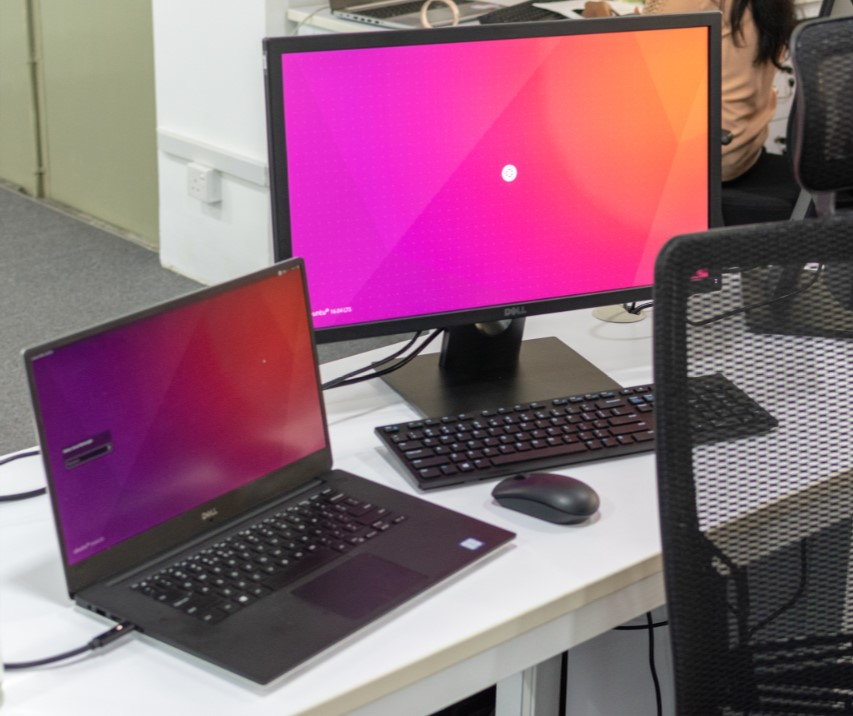
\includegraphics[trim=0cm 0cm 0cm 0cm, clip=true,scale=0.5]{figures/workstation.jpg}
    \caption{Typical Wave Computing Workstation\label{Fig:workstation}}\vspace{-4mm}
    \end{figure}

\begin{figure}[H]
    \centering
    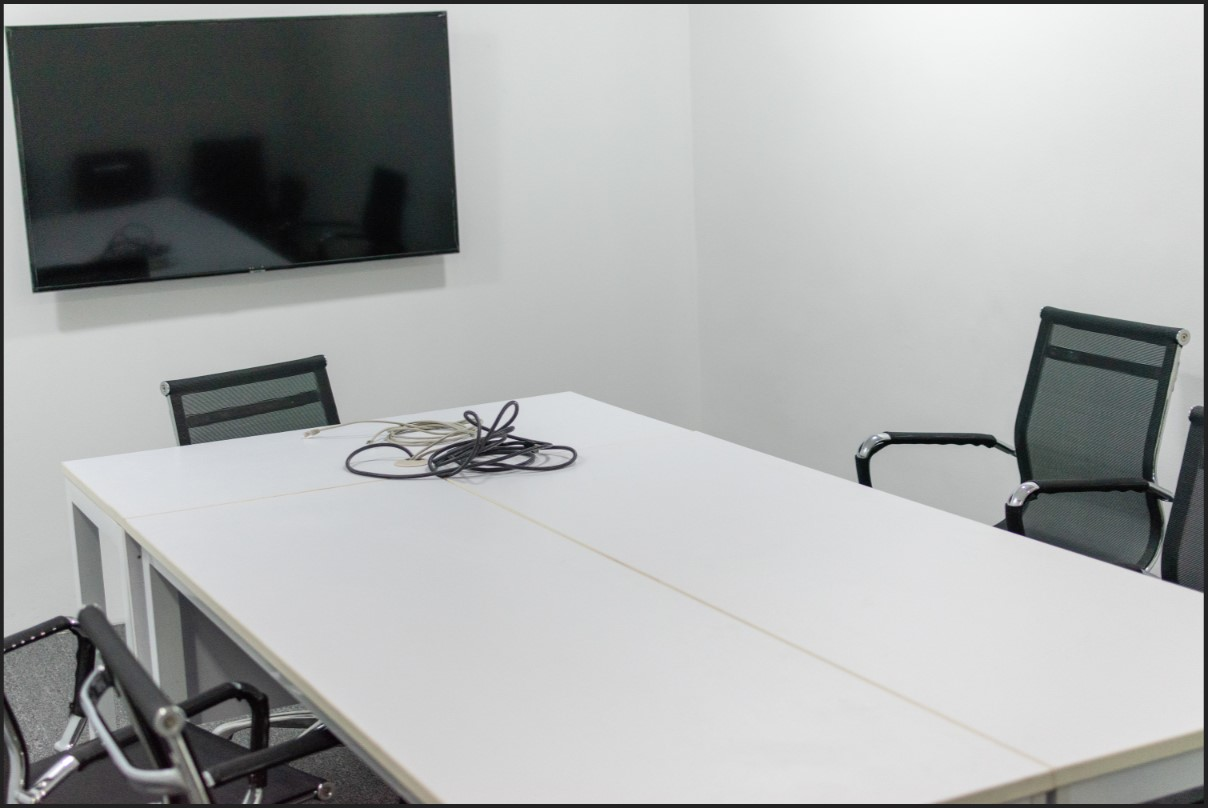
\includegraphics[trim=0cm 0cm 0cm 0cm, clip=true,scale=0.5]{figures/conf_room.jpg}
    \caption{A conference room\label{Fig:confroom}}\vspace{-4mm}
    \end{figure}
    
Wave Computing office provides its employees with state of the art working facilities with a comfortable working space, making it highly productive. There are conference rooms with Large displays that allow almost lifelike meetings with the HQ (Figure~\ref{Fig:confroom}), there are cutting edge workstations (Figure~\ref{Fig:workstation}) and basically everything you can expect from an office. It was absolutely a perfect place to work.

\subsubsection{Supervisor Visits}
\paragraph{}
About once in every 3 months one of the Senior officers from Wave USA comes to Sri Lanka for a direct supervision and review. While we were doing the internship, we had two such visits, both by our team supervisor Eng. Henrik Esbensen. These visits usually consists of individual feedback sessions, project reviews and brainstorm meetings. All of these are highly educational and worthwhile. In these meetings, we would get the chance to present our ideas on how our projects may progress and these ideas are highly respected and almost always accepted. It is customary to end the visit with a dinner in a high class restaurant where they celebrate the progress the company has made.

 